\appendix

\section{Empfindlichkeit}

Es sind die drei Aufnahmen des Oszilloskops f�r den Permanentmagneten im Abstand von 1m, 1.5m und 2m zu sehen.

\begin{figure}[H]
\centering
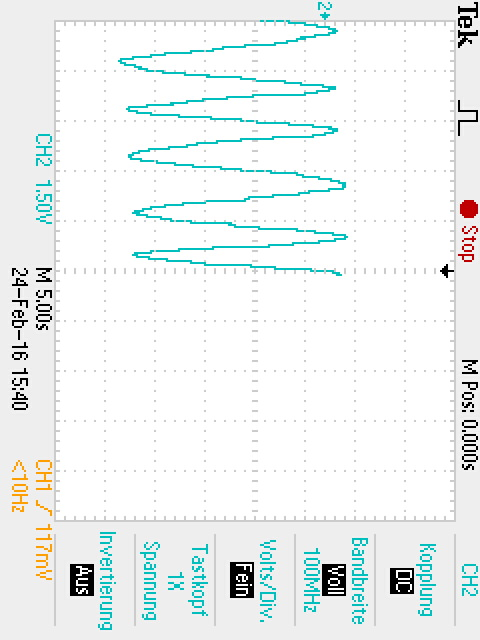
\includegraphics[scale = 0.5,angle=90]{Messungen/TEK0027.JPG}
\caption{Aufnahme der Messspannung bei einem Abstand von 1m}
\label{fig:magnet_1m}
\end{figure}

\begin{figure}[H]
\centering
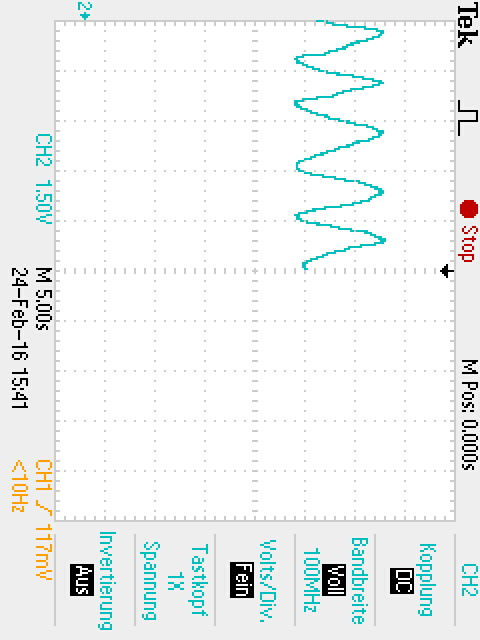
\includegraphics[scale = 0.5,angle=90]{Messungen/TEK0028.JPG}
\caption{Aufnahme der Messspannung bei einem Abstand von 1.5m}
\label{fig:magnet_1.5m}
\end{figure}

\begin{figure}[H]
\centering
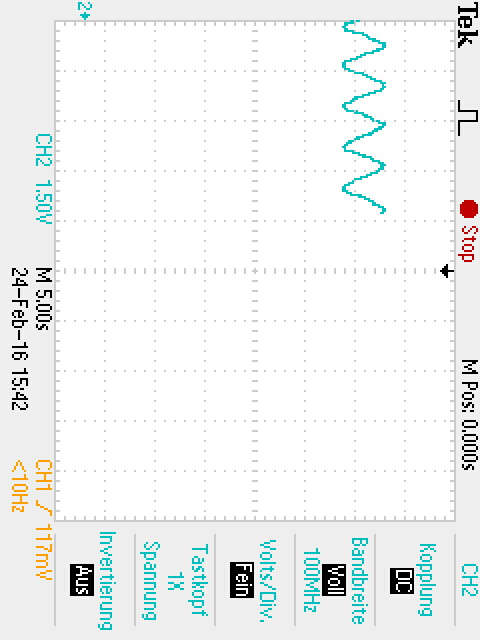
\includegraphics[scale = 0.5,angle=90]{Messungen/TEK0029.JPG}
\caption{Aufnahme der Messspannung bei einem Abstand von 2m}
\label{fig:magent_2m}
\end{figure}